\documentclass[../main.tex]{subfiles}

\begin{document}

\section{Formas de explotación de la vulnerabilidad Log4shell}

Para explotar la vulnerabilida el atacante debe poder acceder a los mensajes que se registran usando \it{Log4J}. En los siguientes apartados se abordarán diferentes formas de explotar la vunlerabilidad \it{Log4Shell}.

Dado que \it{Log4J} se usa en tantos sistemas, esta sección se centrará en los servidores web basados en Java. Además, las explicaciones se acompañarán con algunas pruebas de concepto que se han realizado utilizando un servidor web vulnerable \cite{vulnerable-app}.

%--------------------------------------------------
\subsection{Uso de campos de la cabecera HTTP}

Dada la naturaleza de los servidores web, es muy probable que éstos registren el contenido de diferentes cabeceras HTTP de las peticiones para poder llevar a cabo un análisis estadístico de, por ejemplo, los navegadores con los que ese sitio está siendo accedido (campo \it{User-Agent}). Dado que el contenido de esos campos los fija el usuario que envía la petición, esta es una de las formas más triviales de tener acceso a los mensajes que se vayan a registrar en el servidor web, y por lo tanto, de insertar \it{lookups} que sean interpretados por \it{Log4J}.

%-------------------------
\subsubsection{Campo \it{X-Api-Version}}

La aplicación web vulnerable que se ha utilizado \cite{vulnerable-app} registra usando \it{Log4J} el contenido del campo \it{X-Api-Version} de la cabecera de las peticiones HTTP que recibe. Es por ello que el scanner del apartado anterior lo detectaba como un sitio vulnerable.

Haciendo uso del flag \it{-H} del comando \it{curl} se pueden introducir valores arbitrarios en cualquiera de los campos de la cabecera HTTP. A continuación, se muestra cómo se utiliza para dar un valor concreto al campo \it{X-Api-Version}:
\begin{codigo}{shell}
# Inyección de campo custom llamado X-Api-Version
curl ${IP}:${PORT} -H 'X-Api-Version: field value'
\end{codigo}

A continuación se muestra cómo los valores introducidos son registrados en la traza del servidor web:
\begin{figure}[!h]
\centering
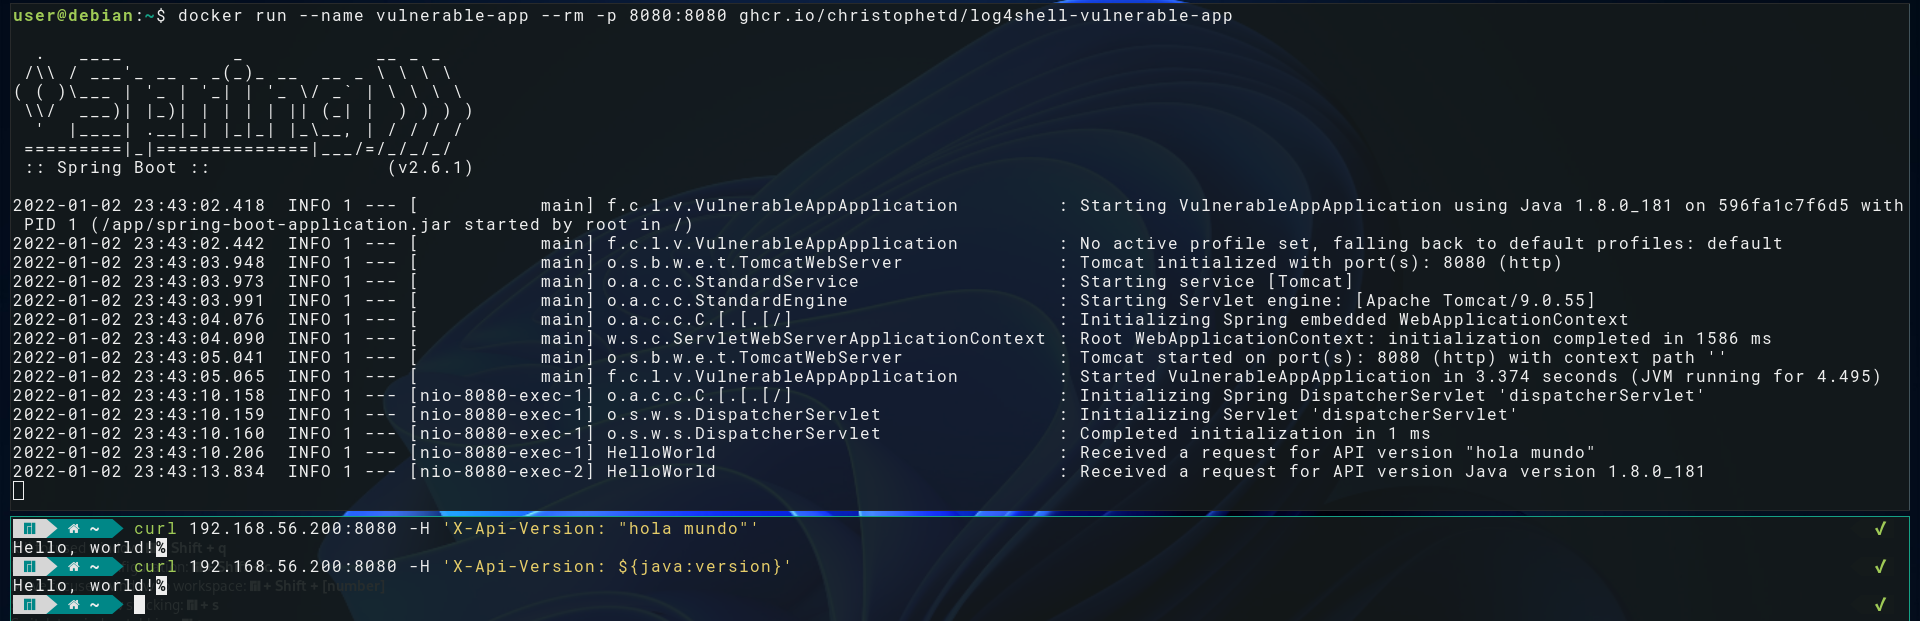
\includegraphics[width=15.0cm]{imagenes/3-Exploit/log4j-lookup_explained.png}
\caption{Introducción de mensajes de log a través del campo 'X-Api-Version'}
\end{figure}

Esta forma de explotación \cite{exploit-lunasec} se utilizará en la siguiente sección para perpetrar un ataque de \it{reverse shell}.

%-------------------------
\subsubsection{Campo \it{User-Agent}}

Otro campo de la cabecera HTTP cuyo valor es fácilmente modificable es \it{User-Agent}. En la práctica 4 ya se utilizó para explotar la vulnerabilidad \it{shellshock}, y en muchos ejemplos que se han encontrado también se aprovechaba para llevar a cabo ataques \it{Log4Shell}.

La forma de darle valor con la herramienta \it{curl} es la siguiente:
\begin{codigo}{shell}
# Inyección como se hizo en la práctica 4
curl ${IP}:${PORT} -A "field value"
# Inyección de la forma análoga a la que se ha realizado con X-Api-Version
curl ${IP}:${PORT} -H 'User-Agent: field value'
\end{codigo}

%--------------------------------------------------
\subsection{Uso de campos de formularios web}

Otra forma de explotación que se ha encontrado durante la realización del trabajo es el uso de los campos de los formularios web.

Si bien se ha visto algún ejemplo que hace uso de ello \cite{exploit-log4shell-formulario}, ésta parece a priori una forma menos realista de acceder a los mensajes de log, pues es menos verosímil que un servidor web registre en su traza el valor de los campos introducidos en los formularios.

\end{document}
